\chapter{Introduction}\label{introduction}

Social media platforms reinforce the risk of toxic behavior, such as hate speech, harassment, and discrimination, compared to traditional media, due to their scale, anonymity, and minimal barriers to community entry \cite{fan:2022,suler:2004,ellison:2007}. While these platforms enable billions to connect and share opinions, their design encourages environments where harmful actions thrive. For instance, the ease of joining online communities encourages rapid aggregation of users \cite{ellison:2007} but also decreases the sense of responsibility, as anonymity reduces social inhibitions \cite{moore:2012,suler:2004,wulczyn:2017}. This dynamic creates fertile ground for toxicity, which spreads easier in digital spaces than in physical interactions \cite{suler:2004}.

\begin{figure}[tb]
  \centering
  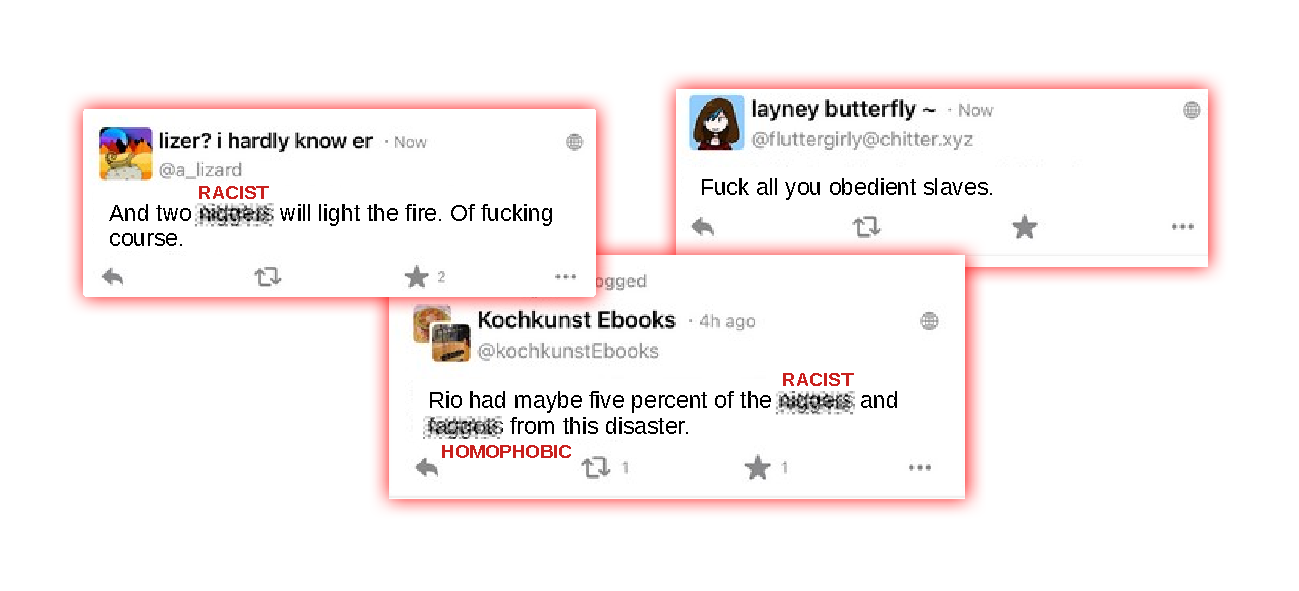
\includegraphics[width=\linewidth]{../material/toxic_comments.pdf}
  \caption{Three toxic toots posted during the 2024 Paris Olympics opening ceremony on Mastodon. The toots contain real content but use invented names for anonymization.}
  \label{toxic-comments}
\end{figure}

Behaviors such as those depicted in Figure~\ref{toxic-comments} disrupt community solidarity and harm individual users, making toxicity a significant challenge for social media platforms \cite{fan:2022,wulczyn:2017}. To mitigate these issues, online communities establish rules and moderation systems to enforce acceptable behavior. Violations of these rules can result in penalties, such as bans or restrictions, depending on the platform's moderation policies \cite{nicholson:2023}.

\begin{figure}[tb]
  \centering
  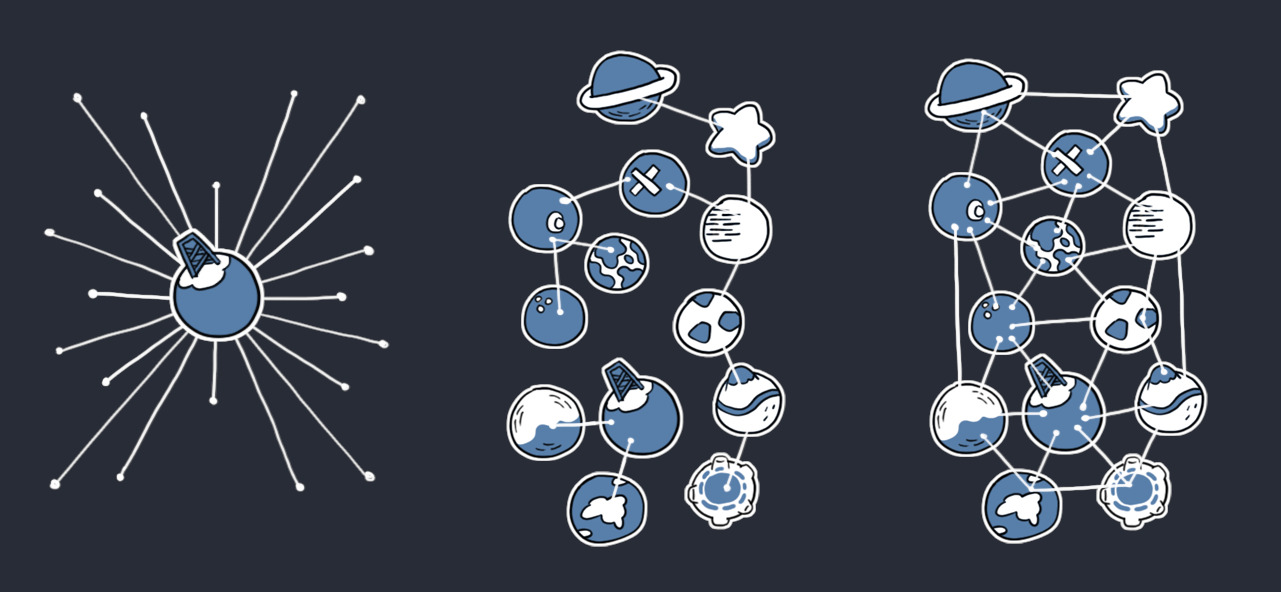
\includegraphics[width=\textwidth]{../material/network_models.jpg}
  \caption[mastodon]{From left to right: Centralized networks connect all through a single controlling hub; Federated networks organize nodes into semi-autonomous interconnected clusters; Distributed networks connect all nodes with multiple pathways. The source of the image is the official Mastodon documentation \cite{mastodon:docs}.}
  \label{network-models}
\end{figure}

To understand the dynamics of toxicity in online communities, this case study focuses on Mastodon\footnote{\url{https://mastodon.social/explore}}, a decentralized alternative to traditional social media platforms like Twitter/X\footnote{\url{https://x.com/}}. The recent acquisition of Twitter/X by Elon Musk has highlighted the risks of centralized social media, where a single individual or entity can exert significant control over platform governance, content moderation, and user experience \cite{he:2023}. Such centralization can lead to abrupt policy changes, increased misinformation, and heightened toxicity, prompting users to seek alternatives. Mastodon, as a decentralized and federated platform, offers a contrasting model where power is distributed across independently operated instances. Like other social media platforms, Mastodon offers the possibility to interact with other people by publishing posts, reacting to posts, or sharing posts. However, Mastodon as a federated social media platform is a decentralized online social networks (DOSN). Federation refers to a special kind of decentralization explained in Figure~\ref{network-models}. Traditional social media platforms, such as Twitter/X, Facebook, or Instagram, are centralized networks and have a single central service that all users access. In contrast, Mastodon has multiple services, called instances, which are used by any number of people. These instances can communicate with each other and create a federated network. Users can freely choose an instance based on language, community rules, moderation policies, and topics of interest. Each instance is managed by its own administrators, who set and enforce local rules \cite{mastodon:docs}. However, this decentralization also introduces unique challenges, such as inconsistent moderation standards and the potential for fragmentation within the fediverse; a network of interconnected but independently operated social platforms. \cite{he:2023}. By examining Mastodon, this study aims to explore how decentralized platforms address toxicity and community management.

\paragraph{Research Gap and Contribution}
Prior work has established foundational knowledge about Mastodon's structure \cite{zulli:2020,la_cava:2021}, moderation practices \cite{bono:2024,nicholson:2023}, and toxicity analysis methods \cite{fan:2022}. However, few studies have systematically investigated toxicity patterns across the mastodon network, and these are limited to small data sets, such as the study by \citet{al-khateeb:2022}. Our research addresses this gap by conducting a large-scale toxicity analysis of Mastodon. We analyzed a 1\% subsample of 15~million Mastodon toots across 724~instances collected throughout 2024. The results reveal two key findings: First, toxicity levels show clear spikes during major political and global events, particularly around the U.S.~election period. Second, active moderation practices significantly lower mean toxicity levels on instances, demonstrating the effectiveness of decentralized moderation approaches.

\enlargethispage{\baselineskip}